\documentclass[../main.tex]{memoir}

\begin{document}

\chapter{Análisis Didáctico}
\label{sec:analisis-didactico}

El conocimiento de los conceptos matemáticos por parte del profesor no garantizan la correcta enseñanza de los mismos. Es necesario un análisis profundo donde, por una parte, se analicen los contenidos a enseñar y su organización; por otra, la situación del alumnado. La unión de estas dos circunstancias guiará al profesor en la elección y diseño de actividades propicias y de un buen método de evaluación. En definitiva, es necesario llevar  a cabo un análisis didáctico. Según \cite{rico2016}, el análisis didáctico es \textit{``el sistema y método de trabajo para el profesor de matemáticas, entre cuyas funciones destaca la reflexión sobre la estructura del currículo de matemáticas, junto con un dominio técnico para planificar e implementar unidades matemáticas escolares''.} \\

En esta sección, abordamos el Análisis de Contenidos, que estudia el sentido de los contenidos y su organización; el Análisis Cognitivo, que se centra en el aprendizaje de un tema matemático por parte de los estudiantes; el Análisis de Instrucción, en el que se deciden y diseñan ejercicios idóneos para el aprendizaje de los contenidos; y el Análisis Evaluativo, como pieza clave para la aplicación de un adecuado sistema de evaluación de lo aprendido.

\section{Análisis de Contenidos}

¿Qué es conocer un concepto matemático? Según \cite{rico2016}, \textit{``conocer su definición, representarlo, mostrar sus operaciones, relaciones y propiedades y los modos de uso, interpretación y aplicación a la resolución de problemas''.} Podemos llevar a cabo este conocimiento por dos vías. La primera, en la que aunamos la estructura conceptual y sus sistemas de representación, generan un significado instrumental del concepto, logrando su dominio por medio de un aprendizaje basado en la memorización de hechos, destrezas y propiedades. Por otra parte, se le puede dar un enfoque funcional, basado en que los conceptos y procedimientos asociados tienen una función y se usan con determinados propósitos. En definitiva, las diversas formas de entender, expresar y usar un concepto constituyen su significado. Por contenido matemático escolarse se entiende un conjunto de conceptos, procedimientos, estructuras y actitudes que los responsables del currículo escogen y organizan, que los profesores comunican y enseñan, para que los escolares aprendan acerca de un tópico matemático escolar determinado y lo utilicen. El análisis del contenido matemático escolar consiste en establecer con detalle sus descriptores y componentes particulares según cada una de las categorías cognitivas de contenido,establecidas por ámbitos y niveles. (\cite{rico2016}). \\

Este análisis se organiza en torno a tres aspectos:

\begin{itemize}
	\item Estructura conceptual. Se relacionan conceptos, procedimientos y actitudes implicados en el contenido objeto de estudio.
	\item Sistemas de Representación. Distintos modos de representación de un concepto matemático de acuerdo a su estructura o sus propiedades.
	\item Sentido. El análisis de contenido se ocupa de estudiar el sentido de un concepto matemático escolar analizando sus términos, contextos, fenómenos y situaciones en lo que se aplica.
\end{itemize}


\subsection{Estructura conceptual}

Según \cite{rico2016}, llamamos \textit{``estructura conceptual al primero de los sistemas de categorías u organizadores que identifica los aspectos formales y los cognitivos con que se caracterizan y describen los contenidos cuyo estudio se considera''}. Como ya comentamos antes, la estructura conceptual se divide en conceptos, procedimientos y actitudes. \cite{rico1997} indica que los conceptos son la sustancia general del conocimiento, aquello que pensamos, mientras que los procedimientos aglutinan los modos actuación y ejecución de tareas matemáticas. Finalmente, el campo actitudinal incluye los aspectos afectivos, éticos y normativos de la disciplina (\cite{rico2016}). Recuperando los contenidos de nuestra unidad didáctica (\cite{RD1105})

\begin{itemize}
	\item Números complejos
	\item Forma binómica y polar
	\item Representaciones gráficas
	\item Operaciones elementales
	\item Fórmula de Moivre.
\end{itemize}

\begin{table}[H]
	\centering
	\begin{tabular}{lcccccc}
		\toprule
		\hspace{2.5cm}Contenido conceptual \\
		\midrule
		- Parte real, parte imaginaria. Unidad imaginaria \\
		- Forma binómica \\
		- Afijo, módulo y argumento de un número complejo \\
		- Conjugado de un número complejo \\
		- Eje real y Eje Imaginario \\
		- Forma polar \\
		- Forma trigonométrica\\
		\bottomrule
	\end{tabular}
	\caption{Conceptos}
	\label{tab:conceptos}
\end{table}


\begin{table}[H]
	\centering
	\begin{tabular}{lcccccccccccc}
		\toprule
		\hspace{4cm}Contenido procedimental \\
		\midrule
		- Identificar la parte real y parte imaginaria de un número complejo \\
		- Calcular el afijo, módulo y argumento de un número complejo \\
		- Calcular el conjugado de un número complejo \\
		- Representar números complejos en su forma binómica y polar\\
		\hspace{0.2cm} en el plano complejo (Eje Real y Eje Imaginario) \\
		- Pasar de forma binómica a forma polar \\
		- Pasar de forma binómica y polar a forma trigonométrica\\
		- Operaciones con números complejos en forma binómica: sumar, \\ \hspace{0.2cm}multiplicar y dividir números complejos. Producto por escalar y potencia. \\
		- Operaciones con números complejos en forma polar: Producto, \\
		\hspace{0.2cm}división, raíz $n$-ésima y potencia. Uso de la fórmula de Moivre.\\
		\bottomrule
	\end{tabular}
	\caption{Procedimientos}
	\label{tab:procedimientos}
\end{table}

\begin{table}[H]
	\centering
	\begin{tabular}{lccccc}
		\toprule
		\hspace{4cm}Contenido actitudinal \\
		\midrule
		- Valoración del cuerpo de los números complejos como el conjunto \\ \hspace{0.2cm} numérico que engloba a los conocidos anteriormente ($\mathbb{N}, \mathbb{Z}, \mathbb{Q}, \mathbb{R}$). \\
		- Valoración de la importancia de los números complejos en ciencia y \\ \hspace{0.2cm} tecnología como en la física cuántica, circuitos electrónicos, \\ \hspace{0.2cm} electromagnetismo o dinámica de fluidos. \\
		\bottomrule
	\end{tabular}
	\caption{Actitudes}
	\label{tab:actitudes}
\end{table}


A su vez, cada concepto relacionada y organiza \textbf{hechos}. Se pueden entender como unidades de información que constituyen un primer nivel básico para analizar el ámbito conceptual de un contenido matemático. El estudio de los hechos se hace mediante cuatro categorías: términos, notaciones, convenios y resultados. Los hechos se relacionan y organizan para dar lugar a \textbf{conceptos} y \textbf{estructuras} (\cite{rico2016}). \\



Concretamente,

\begin{table}[H]
	\centering
	\begin{tabular}{llccccccccccccccccccccc}
		\toprule
		\hspace{5.8cm}\textbf{Hechos} \\
		\midrule
		Términos & Notaciones \\
		\midrule
		- Número complejo & - Forma binómica: $z = a +bi$, $\mathbb{C}$ \\
		& - $i$ unidad imaginaria \\
		- Parte real & - Re $z$ \\
		- Parte imaginaria & - Im $z$ \\
		- Afijo & - $P(a,b)$ punto del plano complejo\\
		- Módulo & - $|z|$ \\
		- Argumento & - $Arg z$ \\
		- Eje real, eje imaginario & \\
		 & - Conjugado: $\bar{z}$ \\
		 & - Forma polar: $z = r_\alpha$ \\
		\midrule
		Convenios & Resultados \\
		\midrule
		- El número complejo $z = a +bi$  & - Todo número complejo $z = a +bi$ \\
		se lee ``a más b i'', eludiéndose & se define como un punto $P(a,b)$  \\
		el signo de multiplicación. & del plano complejo  \\
		- Si $a=0, z$ se dice imaginario puro & - El eje real es el eje de abscisa y el eje \\
		&  imaginario es el eje de ordenadas. \\
		& Los números reales son números  \\
		& complejos con parte imaginaria  \\
		& nula ($b=0$) \\
		\bottomrule
	\end{tabular}
	\caption{Contenido conceptual: Hechos. Términos, notaciones, convenios y resultados}
	\label{tab:terminos-notaciones}
\end{table}


\begin{table}[H]
	\centering
	\begin{tabular}{lccccc}
		\toprule
		\hspace{2cm}Conceptos \\
		\midrule
		- Forma binómica \\
		- Forma polar \\
		- Forma trigonométrica\\
		- Raíz compleja de un polinomio \\
		\bottomrule
	\end{tabular}
	\caption{Contenido conceptual: Conceptos}
	\label{tab:conceptos2}
\end{table}

\begin{table}[H]
	\centering
	\begin{tabular}{lcc}
		\toprule
		\hspace{2.5cm}Estructuras \\
		\midrule
		 - ($\mathbb{C}$,+,·): Cuerpo de los números complejos \\
		\bottomrule
	\end{tabular}
	\caption{Contenido conceptual: Estructuras}
	\label{tab:estructuras}
\end{table}



Por otra parte, en el campo procedimental se diferencian, igualmente, tres niveles, según la complejidad del contenido. Son las \textbf{destrezas}, que procesan hechos; los \textbf{razonamientos}, que procesan conceptos; y las \textbf{estrategias}, que procesan estructuras (\cite{rico2016}). \\

\begin{table}[H]
	\centering
	\begin{tabular}{lcccccc}
		\toprule
		\hspace{5cm}Destrezas \\
		\midrule
		- Identificar la parte real y parte imaginaria de un número complejo \\
		- Calcular el afijo, módulo y argumento de un número complejo \\
		- Calcular el conjugado de un número complejo \\
		- Representar números complejos en su forma binómica y polar\\
		\hspace{0.2cm} en el plano complejo (Eje Real y Eje Imaginario) \\
		- Operaciones con números complejos en forma binómica: sumar, \\ \hspace{0.2cm}multiplicar y dividir números complejos. \\
		- Operaciones con números complejos en forma polar: Producto y \\
		\hspace{0.2cm}división. \\
		\bottomrule
	\end{tabular}
	\caption{Contenido procedimental: Destrezas}
	\label{tab:destrezas}
\end{table}


\begin{table}[H]
	\centering
	\begin{tabular}{lcccccc}
		\toprule
		\hspace{5cm}Razonamientos \\
		\midrule
		- Pasar de forma binómica a forma polar \\
		- Producto por escalar y potencia. \\
		- Pasar de forma binómica y polar a forma trigonométrica\\
		- Cálculo de la raíz $n$-ésima y potencia. Uso de la fórmula de Moivre.\\
		\bottomrule
	\end{tabular}
	\caption{Contenido procedimental: Razonamientos}
	\label{tab:razonamientos}
\end{table}


%% PREGUNTAR POR ESTRATEGIAS
\begin{table}[H]
	\centering
	\begin{tabular}{lcccccc}
		\toprule
		\hspace{5cm}Estrategias \\
		\midrule
		- Estrategias de resolución de problemas con números complejos. \\ \hspace{0.2cm}Aplicaciones a la vida real y uso de software. \\
		\bottomrule
	\end{tabular}
	\caption{Contenido procedimental: Estrategias}
	\label{tab:estrategias}
\end{table}


%% MAPA CONCEPTUAL --> PREGUNTAR

\subsection{Sistemas de Representación}

Comprender un concepto matemático, o una estructura en su totalidad, requiere que el alumno lo recree en su mente por medio de imágenes o representaciones más o menos abstractas. Dichas representaciones deben ser lo más ricas y variadas posibles, para así garantizar la correcta interpretación y captar, en sentido amplio, la naturaleza del concepto objeto de estudio. Concretamente, según \cite{rico2016}, un sistema de representación \textit{``constituye un conjunto estructurado de notaciones, símbolos y gráficas, dotado de una serie de reglas y convenios que permiten expresar determinados aspectos y propiedades de un concepto matemático''}. Por su parte, \cite{lupi2013} señala que cada sistema de representación destaca alguna peculiaridad del concepto que expresa y facilita el entendimiento y trabajo de alguna de sus propiedades. Por todo ello, proponemos cuatro sistemas de representación distintos en torno a un número complejo. Son las siguientes: representación numérica, simbólica o algebraica, representación verbal, representación gráfica y la representación por medio de recursos digitales. 

\subsubsection{Representación numérica, simbólica o algebraica}

En primer lugar, entendemos el cuerpo de los número complejos, $\mathbb{C}$, simbólicamente como 

$$\mathbb{C} = \{a+bi, \forall a,b \in \mathbb{R}\}$$

siendo $i = \sqrt{-1}$. Por tanto, todo número complejo $z$, dados $a,b \in \mathbb{R}$, se puede expresar como

$$z = a+bi, \hspace{1cm} \text{Re }z = a, \text{ Im }z = b$$

Esta representación es llamada forma binómica de un número complejo. No obstante, los números complejos se pueden representar simbólicamente de otras formas. Si llamamos $r = |z|$ y $\alpha = $ Arg $z$, entonces $z = r_{\alpha}$ (forma polar o módulo-argumental de un número complejo). \\

Finalmente, dada la forma binómica y polar, si $a = r \cos \alpha, b=r \sin \alpha$, la forma trigonométrica de un número complejo $z$ se escribe como

$$ z = a + bi = r \cos \alpha + (r \sin \alpha) i = r(\cos \alpha + i \sin \alpha)$$

\subsubsection{Representación verbal}

Habitualmente, los números complejos (también conocidos como imaginarios) se representan verbalmente por medio de la lectura de su forma binómica. Tal y como se indicó en los convenios de la sección anterior, el signo de multiplicación entre la parte imaginaria y la unidad imaginaria se obvia, por lo que, por ejemplo, para el número $z = 5+3i$, se representa verbalmente como ``cinco más tres i''. Por otra parte, se puede expresar el mismo número complejo a través de su forma polar indicando el módulo y argumento. En nuestro ejemplo, $z = \sqrt{34}_{30.96º}$ como ``número complejo con módulo raíz de 34 y argumento 30.96º''.

\subsubsection{Representación gráfica}

Todo número complejo se puede representar en el diagrama de Argand (\cite{argand1971}) o plano complejo (\cite{whittaker1927}). Dada la similitud absoluta con $\mathbb{R}^2$ en cuanto a este aspecto, dado que un número complejo se representa como un vector bidimensional, la representación gráfica es clave para la correcta comprensión por parte del alumno del bloque que nos ocupa. No obstante, también se puede utilizar otro tipo de representaciones para mostrar, por ejemplo, que todos los conjuntos numéricos conocidos son subconjunto del cuerpo de los números complejos. Es decir, que $\mathbb{N} \subset \mathbb{Z} \subset \mathbb{Q} \subset \mathbb{R} \subset \mathbb{C}$. 

\begin{figure}[H]
	\centering
	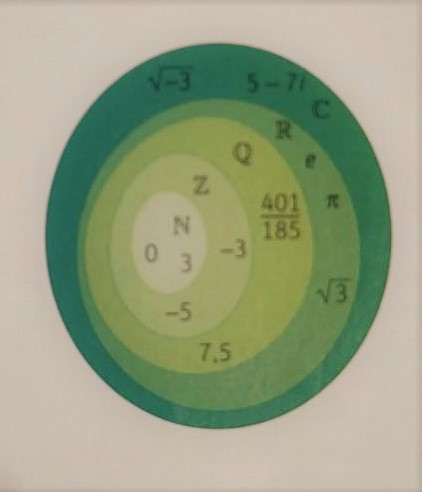
\includegraphics[scale=0.3]{images/complex.jpg}
	\caption{$\mathbb{C}$ como un todo}
	\label{representacion1}
\end{figure}

Asimismo, presentamos el plano complejo o diagrama de Argand y la representación de un número complejo en forma binómica, mostrando su afijo, módulo y argumento.
\begin{figure}[H]
	\centering
	\begin{subfigure}{0.48\textwidth}
		\centering
		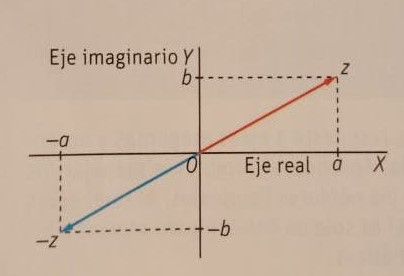
\includegraphics[width=\linewidth]{images/ejes.jpg}
		\caption{Eje Real y Eje Imaginario}
	\end{subfigure}
	\begin{subfigure}{0.48\textwidth}
		\centering
		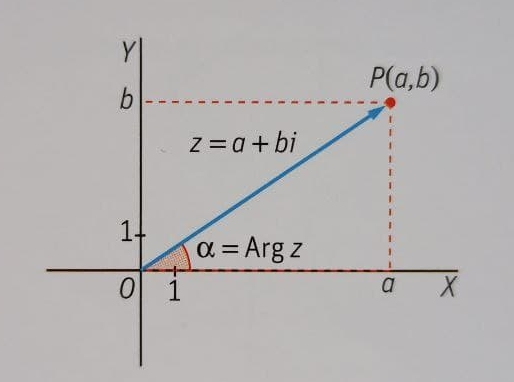
\includegraphics[width=\linewidth]{images/afijo.jpg}
		\caption{Afijo, módulo y argumento}
	\end{subfigure}
	\label{fig:representacion2}
\end{figure}

Finalmente, representamos un número complejo en su forma polar y trigonométrica.

\begin{figure}[H]
	\centering
	\begin{subfigure}{0.48\textwidth}
		\centering
		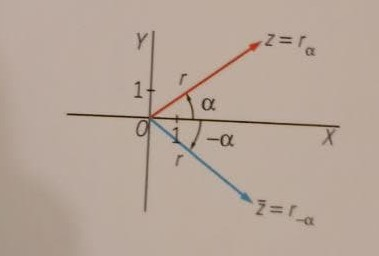
\includegraphics[width=\linewidth]{images/polar.jpg}
		\caption{Forma polar}
	\end{subfigure}
	\begin{subfigure}{0.48\textwidth}
		\centering
		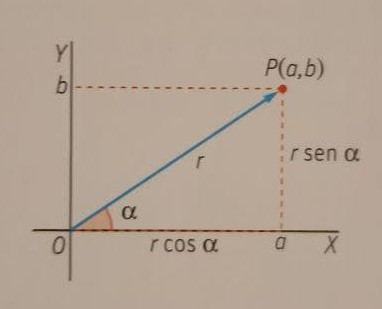
\includegraphics[scale=0.39]{images/trigonometrica.jpg}
		\caption{Forma trigonométrica}
	\end{subfigure}
	\label{fig:representacion3}
\end{figure}

\subsubsection{Recursos digitales}

Existen multitud de recursos digitales, lenguajes de programación y software para representar y trabajar con números complejos. Destacamos aquellos que son software libre y/o herramientas gratuitas y de libre disposición para los alumnos. Gráficamente, Geogebra tiene un material muy extenso, interactivo y variado sobre números complejos. Se puede encontrar en \cite{materialgeogebra}.

\begin{figure}[H]
	\centering
	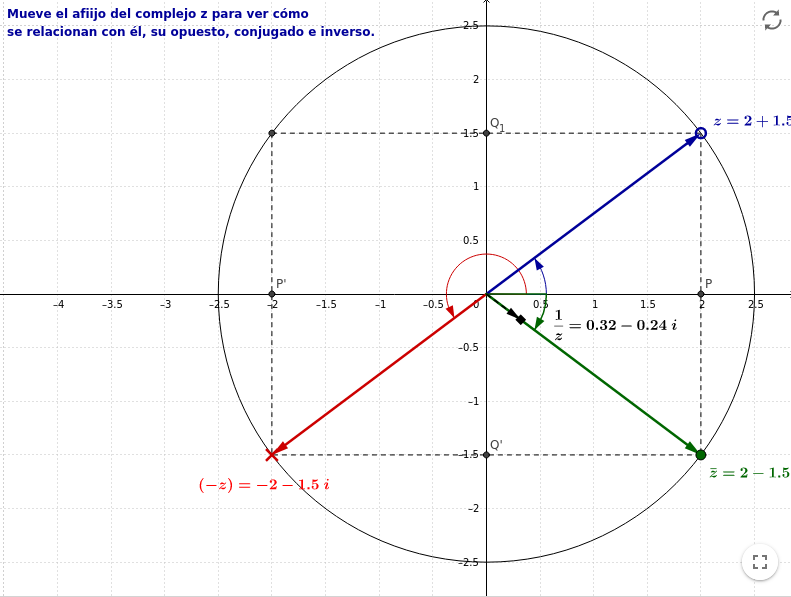
\includegraphics[scale=0.3]{images/conjugado.png}
	\caption{Representación de números complejos en forma binómica. Conjugado, inverso y opuesto}
	\label{geogebra1}
\end{figure}

\begin{figure}[H]
	\centering
	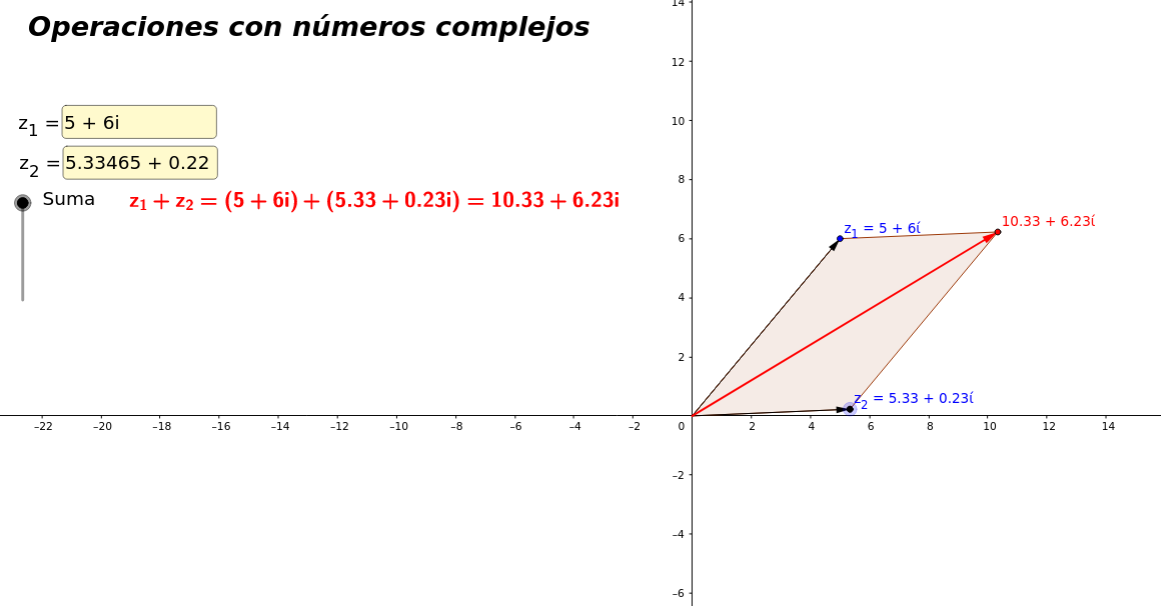
\includegraphics[scale=0.25]{images/sumar.png}
	\caption{Operaciones interactivas con números complejos. En el ejemplo, sumar}
	\label{geogebra2}
\end{figure}


\begin{figure}[H]
	\centering
	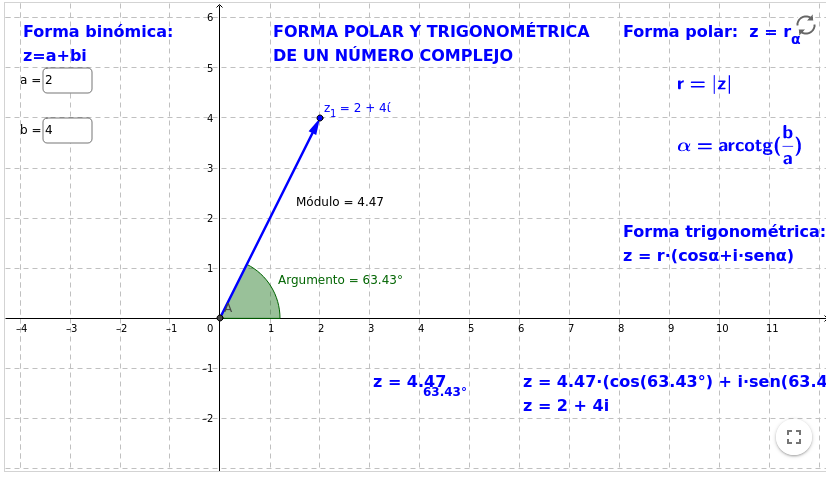
\includegraphics[scale=0.3]{images/polar.png}
	\caption{Representación en forma polar}
	\label{geogebra3}
\end{figure}

Lenguajes de programación más dedicados (como Maxima CAS, wxMaxima) o de propósito general (Python) y herramientas como WolframAlpha (gratuita en su versión básica) son alternativas interesantes para la representación de números complejos. Incluso es posible trabajar con números complejos en calculadoras científicas.

\subsection{Sentido del Concepto Matemático}

Tal y como indica \cite{rico2016}, los conceptos matemáticos alcanzan su máxima expresión cuando se piensa con plenitud su sentido, la cual se logra cuando se entienden sus diferentes modos de uso, se aplican en variedad de situaciones, se comprenden los tipos de problemas que resuelven, se dominan los términos propios del concepto y se conocen los fenómenos que organizan. Estos aspectos serán desarrollados en la presente sección con la intención de completar el dominio de su significado. 

\subsubsection{Términos}

El estudio de una disciplina viene determinado por el conocimiento del estudiante del campo semántico subyacente a dicha disciplina. En general, es muy relevante poseer un gran número de sinónimos en torno a términos relacionado con conceptos, de manera que queden correctamente identificados y caracterizados. No obstante, el origen de los términos utilizados es relevante a la hora de garantizar el aprendizaje del alumnado. \cite{rico2016} señala que si los términos son parte del patrimonio lingüístico del estudiante, el modo de uso del concepto relacionado está condicionado por este bagaje. Si se está explicando un concepto matemático nuevo, es crucial conocer qué términos conocen los estudiantes y, si se da el caso en el que el alumno conoce el término pero no la acepción propia al concepto matemático, es necesario reconducir su asociación de ideas para que el término ahora también tenga sentido en el ámbito matemático. Un claro ejemplo es la palabra \textit{determinante}. Cuando un alumno llega a segundo de bachillerato, el término \textit{determinante} es bien conocida para él (o ella): primero, como un adjetivo que califica a un sustantivo como importante o que determina. Por otra parte, también están familiarizados con la acepción de \textit{determinante} como elemento gramatical (como un artículo). Sin embargo, no conoce la acepción matemática, por lo que al principio le resultará poco familiar relacionar el término \textit{determinante} con teoría de matrices. Es trabajo del profesor ``tender puentes'' entre los campos semánticos del alumno y así afianzar con todas las garantías el concepto matemático objeto de estudio. \\

En nuestro bloque de contenidos tenemos ciertos términos que serán totalmente novedosos para los alumnos desde la perspectiva matemáticas pero sí familiares en su vocabulario cotidiano. Partimos del nombre \textit{número complejo}, que ya de por sí puede crear rechazo o falta de confianza en el estudiante. Complejo, como algo difícil, complicado o enmarañado; o como un conjunto de establecimientos industriales próximos, no parece ser un término muy cómodo para presentar un cuerpo matemático. La alternativa tampoco es mucho mejor, \textit{número imaginario}, puesto que el alumno puede entender que son una invención o elementos sin mucha importancia. Desligar esos significados comunes, en mi opinión casi peyorativos, y que podrían generar estigma o rechazo, es clave para que los alumnos estudien estos contenidos sin prejuicios. \\

Otro término importante es forma \textit{polar} que realmente deriva del sistema de representación en Coordenadas Polares (\cite{adams2013}). En mi opinión, durante la explicación del concepto de forma polar la mención de las coordenadas polares y su historia puede ser idónea, invitando al alumnado a conocer un poco más la historia de la Matemática. \\

Por último, podemos señalar \textit{argumento} como un término quizá ligeramente conocido en el ámbito matemático y ampliamente extendido en el lenguaje coloquial como un razonamiento para probar una proposición o para convencer, frente al ámbito de los números complejos, donde el argumento es el ángulo que forma dicho número con el eje real.

\subsubsection{Contextos Matemáticos}

Los contextos en los que los números complejos tienen cabida están muy ligados al desarrollo científico-tecnológico. Como ya he comentado, se aplican en física y química avanzada (cuántica) y en multitud de tecnologías actuales, como los túneles de viento para la fabricación, diseño y control de calidad de vehículos (dinámica de fluidos). No obstante, podemos decir que la interacción más directa entre la sociedad, y por ende el alumnado, y los números complejos es el electromagnetismo. Además, los estudiantes de Bachillerato, a través de asignaturas como Física I, Física II o Tecnología Industrial estudiarán en profundidad el campo eléctrico y magnético, acercándose a los circuitos y, en particular, a los circuitos de corriente alterna. Sabemos que la corriente alterna se forma con ondas sinusoidales periódicas con expresión:

$$V(t) = V_0  \sin(\omega t + \varphi)$$

con $V_0$ la amplitud máxima, $\omega$ la frecuencia angular y $\varphi$ el desfase. Dicha expresión se puede representar por medio de números complejos como

$$V(t) = V_0 \cos(\omega t +\varphi) + V_0 \sin(\omega t + \varphi) i = V_0 e^{(\omega t + \varphi)i}$$

En consecuencia, se puede escribir la ley de Ohm generalizada por medio de la división compleja, base de cálculo en todos los circuitos electrónicos. En definitiva, los números complejos son absolutamente necesarios en nuestra vida diaria y es posible, por medio de conexiones con otras asignaturas, justificar el contexto matemático de los mismos.
\subsubsection{Fenómenos}

Tal y como expresa \cite{lupi2013} en \cite{rico2013}, la historia es un buen mecanismo para estudiar el contenido de un tema, pues el desarrollo histórico es útil para determinar el origen de los conceptos, comparar sistemas de representación o localizar problemas clásicos. \\

Por sorprendente que pueda parecer, los números complejos surgieron por la necesidad de resolver ecuaciones cúbicos y no cuadráticas. Hagamos un recorrido por la historia de los números complejos: \\

Entre los años 780-850, Al-Khwarizmi plasmaba en \textit{Álgebra} soluciones para ecuaciones cuadráticas de varios tipos. Dichas soluciones coinciden con lo que se aprende en los colegios hoy día si nos restringimos únicamente a soluciones positivas (\cite{waerden1985}). Las pruebas que se propusieron están basadas en geometría. Las fuentes parecen provenir de la matemática hindú y griega. En palabra de \cite{waerden1985}, \\

``Bajo el califato de al-Ma'mum (813-833), al-Khwarizmi formó parte de la \textit{Casa de los Sabios}, una especie de academia de científicos fundada en Bagdad, donde se hubo una gran tradición de aprendizaje e investigación científica.'' \\

Los métodos algebraicos conocidos por los árabes fueron recuperados en Italia gracias a la traducción al latín del álgebra desarrollada por al-Khwarizmi por Gerard de Cremona (1114-1187), y por los trabajos de Leornado de Pissa (Fibonacci) (1170-1250). \\

Sobre el año 1225, cuando Federico II reinaba en Sicilia, Leonardo de Pisa se presentó ante el emperador (\cite{nahin1998}). Ciertos matemáticos locales le propusieron problemas que Leonardo resolvió sin dificultad. Uno de esos problemas fue encontrar la solución de la ecuación

$$x^3+2x^2+10x=20$$

La ecuación cúbica en su forma general

$$ x^3+ax^2+bx+c = 0$$

se puede reducir a una forma más simple

$$x^3+px+q = 0$$

a través del cambio de variable $x'  = x + \frac{1}{3}a$. Este cambio de variable apareció por primera vez en dos manuscritos florentinos anónimos al final del siglo XIV. \\

Si se restringen los valores posibles para $x$ a los positivos, surgen tres casos conocidos como \textit{cúbicas deprimidas}:

$$ (a) \hspace{1cm} x^3+px = q $$
$$ (b) \hspace{1cm} x^3 = px+q $$
$$ (c) \hspace{1cm} x^3+q = px $$

El primero en resolver la ecuación (a) (y quizá (b) y (c)) fue Scipione del Ferro, profesor de la Universidad de Bolonia hasta que falleció en 1526 (\cite{mactutor}). En su lecho de muerte, del Ferro confió la fórmula a su alumno Antonio María Fiore. Fiore retó a Tartaglia a un concurso matemático. La noche antes del concurso, Tartaglia redescubrió la fórmula y ganó el concurso. Tartaglia, por su parte, reveló la fórmula (pero no la demostración) a Gerolamo Cardano, quien firmó una cláusula de confidencialidad. Sabiendo la fórmula, Cardano fue capaz de encontrar la demostración. Más tarde, Cardano supo que del Ferro tenía la fórmula y la verificó. Entonces, Cardano procedió a publicar la fórmula para los tres casos en su \textit{Ars Magna} (1545). Se sabe que Cardano mencionó a del Ferro como primer autor y a Tartaglia como un matemático que encontró la fórmula de manera independiente. \\

Una dificultad del caso (b) que no fue presentada en la solución de (a) se basa en la posibilidad de tener una raíz cuadrada de un número negativo en la expresión numérica de la fórmula. Por ejemplo, sustituyendo $x = u+v$ en $x^3=px+q$ para obtener

$$ x^3-px = u^3+v^3+3uv(u+v)-p(u+v) = q$$

Sea $3uv = p$ para obtener $u^3+v^3 = q$ y $u^3 v^3=(p/3)^3$. Es decir la suma y el producto de dos cubos es conocida. Esto se utiliza para formar una ecuación cuadrática que se puede resolver

$$ x = u+v = \sqrt[3]{\frac{1}{2}q+w} + \sqrt[3]{\frac{1}{2}q-w}$$

donde 

$$ w = \sqrt{(\frac{1}{2}q)^2-(\frac{1}{3}p)^2}$$

El llamado \textit{casus irreducibilis} se da cuando la expresión bajo el signo radical $w$ es negativo. Cardano elude discutir ese caso en \textit{Ars Magna}. Quizá, en su mente, evitarlo estaba justificado por la correspondencia, ahora sabemos incorrecta, entre el \textit{casus irreducibilis} y la ausencia de una solución real y positiva para la cúbica. \\

Según \cite{waerden1985}, ``Cardano fue el primero en introducir números complejos de la forma $a + \sqrt{b}$ desde el punto de vista del álgebra, pero tenía reticencias sobre ello''.\\

Rafael Bombelli escribió un compendio de tres libros, entre 1572 y 1579, llamado \textit{l'Algebra}. Bombelli introdujo la notación de $\sqrt{-1}$, llamándolo \textit{piú di meno}. La discusión sobre cúbicas en \textit{l'Algebra} sigue los trabajos de Cardano, pero ahora el \textit{casus irreducibilis} se discute concienzudamente (\cite{blank1999}). Bombelli consideró la ecuación

$$ x^3 = 15x+4$$

para la cual la fórmula de Cardano dice

$$ x = \sqrt[3]{2+\sqrt{-121}} + \sqrt[3]{2-\sqrt{-121}}$$

Bombelli observó que la ecuación cúbica tiene $x = 4$ como solución, y a continuación explica la expresión dada por la fórmula de Cardano a través de otra expresión de $x = 4$. Estableciendo

$$ \sqrt[3]{2+\sqrt{-121}} = a +bi$$

de donde se deduce

$$ \sqrt[3]{2-\sqrt{-121}} = a-bi$$

y se obtiene, tras manipulaciones algebraicas, $a=2$ y $b=1$. Por tanto,

$$x = a+bi +a -bi = 2a = 4$$

René Descartes (1596-1650) fue un filósofo cuyo trabajo, \textit{La Géométrie} (\cite{descartes1952}), incluye su aplicación del álgebra a la geometría de donde obtenemos hoy día la geometría cartesiana. Descartes fue presionado por sus ideas para publicar sus ideas, y escribió un tratado de ciencias con título \textit{Discours de la méthod pour bien conduire sa raison et chercher la vérité dans les sciences}. En él, Descartes asoció los números imaginarios con imposibilidades geométricos. Esto se puede ver por la construcción geométrica que usó para resolver la ecuación $z^2 =az-b^2$, con $a$ y $b^2$ positivos. \\

John Wallis (1616-1703) propuso en su trabajo \textit{Algebra} que los números negativos tenían una perfecta explicación física, basada en una recta con una marca en el cero, de manera que los números positivos miden la distancia desde el cero a un punto a su derecha, y los números negativos como una distancia al cero por la izquierda. Igualmente, hizo un gran progreso en la interpretación geométrica de $\sqrt{-1}$.  \\

Abraham de Moivre (1667-1754) conoció a Newton y en 1698 mencionó que Newton ya conocía, antes de 1676, una expresión equivalente a la actual fórmula de Moivre:

$$(\cos \theta + i \sin \theta))^n = \cos(n\theta) + i \sin(n \theta)$$

donde $n$ es un entero. Aparentemente Newton usó esta fórmula para calcular las raíces cúbicas que aparecían en la fórmula de Cardano, en el caso irreducible. de Moivre sabía y usó la fórmula que lleva su nombre, ya que se ve claro en sus trabajos, aunque nunca la escribió explícitamente. \\

L. Euler (1707-1783) introdujo la notación $i = \sqrt{-1}$ (\cite{dunham1999}), y visualizó los números complejos con coordenadas rectangulares. Euler usó la fórmula $x+iy = r(\cos \theta +i \sin \theta)$, y representó las raíces de $z^n = 1$ como los vértices de un polígono regular. Definió la exponencial compleja y probó la identidad $e^{i\theta} = \cos \theta +i \sin \theta$. \\

Caspar Wessel (1745-1818) fue el primero en obtener y publicar una representación apropiada de los números complejos. En 1797, Wessel presentó su artículo \textit{On the Analytic Representation of Direction: An Attempt} en la Real Academia de las Ciencias de Dinamarca. En él se presentaba lo que hoy llamamos vectores (\cite{crowe1967}). Utilizaba la suma geométrica de vectores (ley del paralelogramo) y definió la multiplicación de vectores en términos de lo que hoy llamamos multiplicar números complejos en su forma polar: sumando sus argumentos y multiplicando sus módulos. \\

Jean-Robert Argand (1768-1822) escribió un trabajo llamado \textit{Essay on the Geometrical Interpretation of Imaginary Quantities} (\cite{argand1971}) pero no consiguió publicarlo. Una copia cayó en manos del matemático A. Legendre (1752-1833). Este lo publicó en 1813 en \textit{Annales de Mathématiques} donde se asentaron las bases de los números y el plano complejo. \\

William Rowan Hamilton (1805-1865) definió en 1831 números reales relacionados $(a,b)$ como parejas. Además, introdujo la suma de dos parejas $(a,b) + (c,d) = (a+c,b+d)$ y la multiplicación $(a,b)(c,d) = (ac-bd,bc-ad)$. Es decir, presentó las operaciones algebraibas elementales de números complejos. \\

Se cree que Carl Friedrich Gauss (1777-1855) ya poseía una representación geométrica de los números complejos en 1796, pero no la publicó hasta 1831, cuando envió su ideas a la Real Sociedad de Gottingen. Gauss introdujo el término número complejo. \\

Augustin-Louis Cauchy (1789-1857) inició la teoría de funciones complejas en un trabajo de 1814. El término de función analítica no se mencionaba, pero el concepto se percibía. El trabajo fue publicado en 1825. La integral curvilínea aparece en él, pero no por primera vez, ya que Poisson había publicado en 1820 un artículo con un recorrido que no era en línea recta. Cauchy construyó el conjunto de los números complejos en 1847 como $R[x]/(x^2+1)$. \\

Hoy en día, la variable compleja sustenta los mayores avances en ciencia y tecnología conocidos, como la física cuántica, la química cuántica, los circuitos electrónicos, electromagnetismo o la  dinámica de fluidos.


\subsubsection{Situaciones}

Como sabemos, el marco teórico del estudio PISA considera cuatro tipo de situaciones: Personales, Laborales, Sociales y Científicas. Los números complejos están restringidos al ámbito científico y laboral (o educativo) si el nivel de especialización del alumno/a sigue caminos científico-tecnológicos. En particular, en la física cuántica, la química cuántica, los circuitos electrónicos, electromagnetismo o la dinámica de fluidos, con aplicaciones sobre la ingeniería eléctrica o del automóvil (túnel de viento). En el nivel de 1º Bachillerato, es complicado que los estudiantes se encuentren con los números complejos en sus situaciones cotidianas, a pesar del gran impacto que la variable compleja tiene en el día a día del ser humano.


\section{Análisis Cognitivo}

A continuación, presentamos el análisis cognitivo, es decir, nos centraremos en estudiar cuál es el cometido de aprender los contenidos que hemos enunciado. Para ello, estudiamos las expectativas de aprendizaje, esto es, qué se espera que los escolares aprendan; las limitaciones en el aprendizaje, es decir, qué puede ralentizar, bloquear o dificultar ese aprendizaje, distinguiendo entre las dificultades subyacentes y los errores que habitualmente se cometen; y la oportunidades de aprendizaje, en otras palabras, cómo se puede promover el aprendizaje y minimizar el impacto de esas limitaciones (\cite{rico2016}, \cite{lupi2013}).

\subsection{Expectativas de aprendizaje}

Teniendo en cuenta todos los aspectos expresados en el análisis de contenido, los objetivos específicos de esta unidad son los siguientes:

\begin{itemize}
	\item \textbf{O1.} Valorar los números complejos como ampliación del concepto de número real.
	\item \textbf{O2.} Conocer un número complejo en su forma binómica, distinguiendo y calculando su afijo, módulo, argumento y conjugado.
	\item \textbf{O3.} Manejar la forma polar y trigonométrica de un número complejo. Transformaciones entre distintas formas de representación.
	\item \textbf{O4.} Representar gráficamente números complejos en su forma binómica, polar y trigonométrica.
	\item \textbf{O5.} Operar con números complejos: suma, resta, multiplicación, división y potencia.
	\item \textbf{O6.} Obtener soluciones complejas en ecuaciones de segundo grado con coeficientes reales.
	\item \textbf{O7.} Utilizar la fórmula de Moivre en el caso de potencias.
	\item \textbf{O8.} Comprender y valorar la historia así como la importancia actual de los números complejos.
	\item \textbf{O9.} Utilizar software libre para operar y representar números complejos.
\end{itemize}

El proyecto PISA/OCDE definió las componentes de la competencia matemática (\cite{pisaocde}). Son las siguientes: Razonar y argumentar (\textbf{RA}), Comunicar (\textbf{C}), Matematizar (\textbf{M}), Diseñar estrategias para resolver problemas (\textbf{RP}), Representar (\textbf{R}), Utilizar operaciones y lenguaje simbólico (\textbf{LS}) y Usar herramientas matemáticas (\textbf{HM}). \\

Por todo ello, en la siguiente tabla indicamos qué competencias matemáticas PISA se desarrollan con los objetivos específicos anteriormente comentados.

\begin{table}[H]
	\centering
	\begin{tabular}{lcccccccc}
		\hline
		\toprule
		\textbf{Objetivos específicos} & \textbf{RA} & \textbf{C} & \textbf{M} & \textbf{RP} & \textbf{R} & \textbf{LS} & \textbf{HM} \\ 
		\midrule
		O1                             & X           & X          & X          &             & X          & X           &             \\ \hline
		O2                             &             & X          & X          &             & X          & X           &             \\ \hline
		O3                             & X           &            & X          & X           &            & X           & X           \\ \hline
		O4                             &             & X          &           & X           & X          & X           & X           \\ \hline
		O5                             & X           &            &          & X           &            & X           & X           \\ \hline
		O6                             & X           & X          & X          & X           &            & X           & X           \\ \hline
		O7                             & X           &            & X          & X           &            & X           &             \\ \hline
		O8                             & X           & X          & X          &             &            &             &             \\ \hline
		O9                             & X           & X          & X          & X           & X          & X           & X           \\ 
		\bottomrule
	\end{tabular}
	\caption{Objetivos específicos y su relación con las competencias PISA/OCDE}
	\label{tab:obj-pisa}
\end{table}

Como se pude comprobar, las competencias más desarrolladas por nuestra actividad son Razonar y Argumentar, Matematizar y Uso de Lenguaje Simbólico. Resolver problemas y Comunicar van muy de la mano. Por último, cabe destacar que pretendemos reforzar en el alumnado tanto la metodología tradicional como el uso de software a la hora de resolver problemas específicos o hacer representaciones.

\subsection{Limitaciones en el aprendizaje}

Las expectativas de aprendizaje mencionadas se pueden ver ralentizadas o mermadas por distintos factores, como la complejidad inherente de los conceptos, el interés del alumnado, la heterogeneidad del grupo, etc. En definitiva, un profesor debe estar preparado para determinar qué dificultades encuentran los estudiantes al enfrentarse un bloque de contenidos y, en consecuencia, qué errores cometen en el proceso de aprendizaje de los mismos y en la realización de ejercicios propuestos. Esta apartado se centra en eso precisamente: determinar las dificultades y los errores más frecuentes cuando se estudian números complejos.


\subsection{Oportunidades de aprendizaje}

\section{Análisis de Instrucción}



\section{Análisis Evaluativo}
\end{document}

%%% Local Variables:
%%% mode: latex
%%% TeX-master: "../main"
%%% End:
